\chapter{Grundlagen}
\label{grundlagen}

Im Folgenden werden die beiden wichtigsten Technologien vorgestellt, die als Grundlage für diese
Arbeit verwendet wurden. Zum einen das Eclipse Modeling Framework, welches die Umgebung für die
gesamte Implementierung darstellt und zum anderen die Modell Transformationssprache Henshin als
wichtigste Technolgie zur Umsetzung des Semantic-Liftings.

\section{Eclipse Modeling Framework}

Das Eclipse Modeling Framework (EMF) ist, wie der Name schon sagt, ein auf Eclipse basierendes
Framework zur Generierung von Quelltext aus Modellen. EMF bildet dabei eine Brücke zwischen
verschiedenen Modellierungsansätzen. Als Eingabe für EMF können z.B. UML-Diagramme, XML-Schemata
oder spezielle Java Interfaces dienen. Damit EMF diese Daten weiter verarbeiten kann, wird dann aus
jedem Eingabemodell ein entsprechendes Modell im EMF eigenen Modelltyp Ecore erzeugt. EMF bietet
aber auch Editoren, in denen Ecore Modelle direkt erzeugt und bearbeitet werden können. Ecore ist
ein s.g. plattformunabhängiges  Metamodell (\textit {engl. platform independent model (PIM)}), d.h.
durch Ecore wird noch nicht festgelegt, für welche Zielplattform später Quelltext generiert werden
soll und wie die konkrete Implementierung des Modells aussehen wird. Eine etwas vereinfachte Form
des Ecore Metamodell ist in Abbildung \ref{fig:ecore_metamodel} zu sehen. Ecore ist eine Implementierung
des EMOF (\textit{Essential Meta Object Facility} \cite{MOF}) Metamodells. EMOF beschreibt einen
Ausschnitt des Metamodells der UML 2.0. Die in Ecore formulierten Modelle dienen nur dazu, die
Datenstrukturen eines Programms zu beschreiben. In der gesamten UML gibt es hingegen aber auch
Modelle, um das Verhalten einer Software zu beschreiben. So wie EMOF ist Ecore ein Modell, welches
sich selbst definiert, d.h. das Metamodell von Ecore ist selbst ein Ecore Modell. Man spricht dann
auch von einem selbstreferentiellen Metamodell.

\begin{figure}[htb]
  \centering
  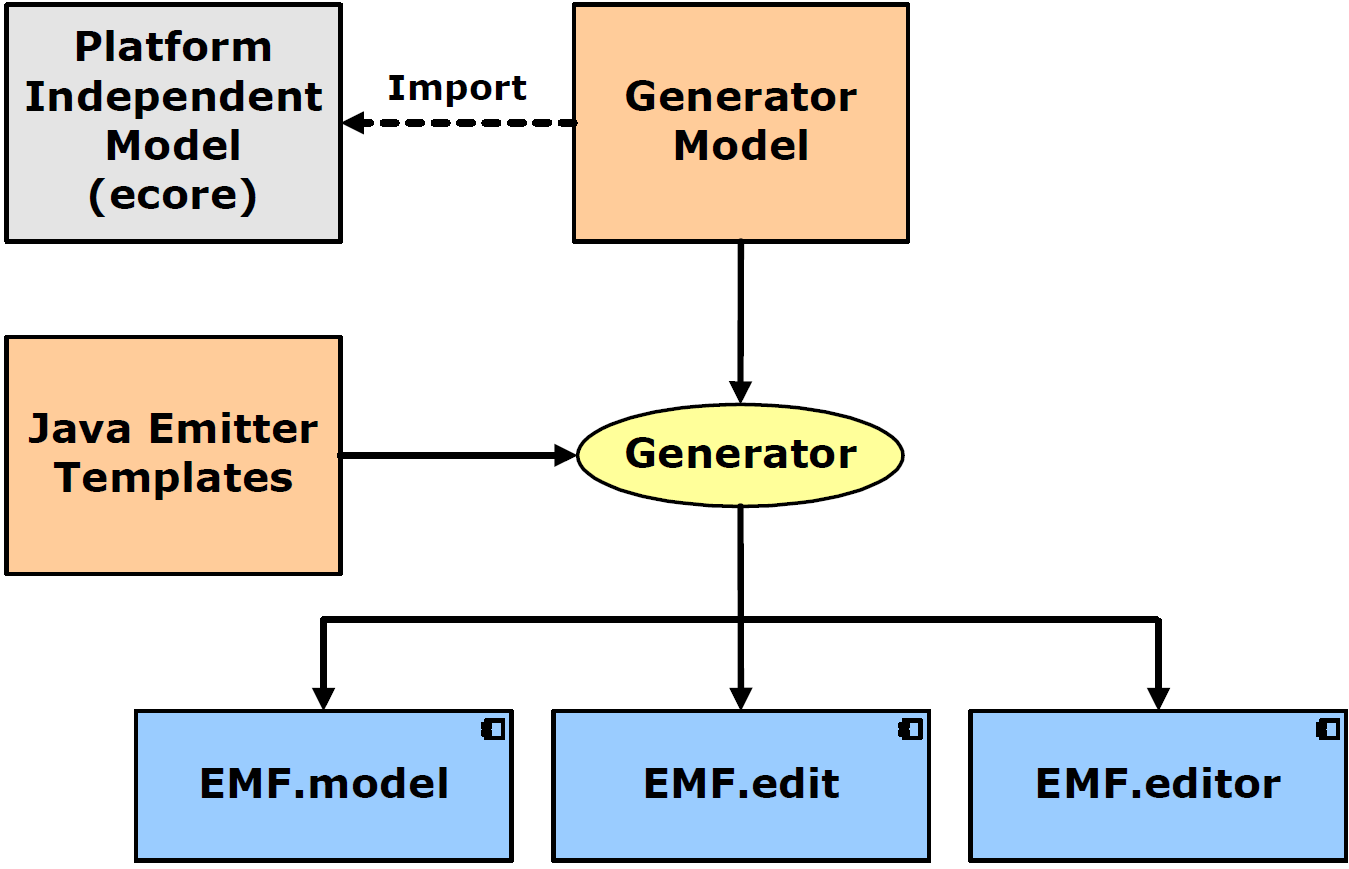
\includegraphics[scale=0.18]{images/emf_toolset.png}
  \caption{"`EMF Toolset from 30.000 Feet"' \cite{EMFCon} (S.7)}
  \label{fig:emf_toolset}
\end{figure}

Wie in Abbildung \ref{fig:emf_toolset} dargestellt, wird neben dem Ecore Modell zur
Quelltext-Gene"-rie"-rung noch ein s.g. Generator Modell (\textit{GenModel}) benötigt. Das Generator
Modell wird weitestgehend automatisch erzeugt und erweitert das plattformunabhängige Ecore Modell um
plattformspezifische Informationen. Das Generator Modell kann vom Benutzer angepasst werden und
steuert direkt die Quelltext Ausgabe des darunter liegenden Generators. Innerhalb des Generators
findet nun eine s.g. Modell-zu-Text Transformation statt, d.h. aus dem Generator Modell wird nun der
eigentliche Quelltext generiert. Dazu werden Java Emitter Templates (JET) verwendet, diese enthalten
Textmuster die vorgeben wie die Modell-Elemente zu transformieren sind. Die Zielsprache von EMF ist
grundsätzlich Java. Theoretisch kann JET aber auch verwendet werden, um einen Generator zu
schreiben, der aus dem plattformunabhängigen Ecore Modell z.B. SQL oder C\# Quelltext erzeugt. In
Abbildung \ref{fig:emf_toolset} sind die drei wichtigsten Pakete zu sehen, die generiert werden
können:

\begin{itemize}
  \item \textbf{EMF.model:} Der hier erzeugte Java Quelltext ist ein s.g. plattformspezifisches
  Modell (\textit{engl. platform specific model (PSM)}). Dieses stellt die Implementierung des zuvor
  in Ecore beschriebenen plattformunabhängigen Modells dar. Der Java Quelltext ist in der Regel
  sofort ausführbar, um als Datenmodell für eine drauf aufbauende Applikation eingesetzt zu werden.
  An gegebenen Stellen kann bzw. muss der Entwickler dann noch eigenen Code einfügen.
  
  \item \textbf{EMF.edit:} Dieses Paket stellt eine Zugriffsschicht zwischen Modell und
  Modell-Editor dar. Zum einen wird durch die Zugriffsschicht festgelegt, welche Befehle der Editor
  auf dem Modell ausführen darf, zum anderen werden die Daten des Modells für den Editor ggf. in
  passender Form aufbereitet. Je nach benötigter Funktionalität kann die Zugriffsschicht dann noch
  an die Gegebenheiten des Editors angepasst werden.
  
  \item \textbf{EMF.editor:} Hier stellt EMF einen einfachen baumbasierten Editor zum Erstellen und
  Bearbeiten von Modell Instanzen zur Verfügung. Der Editor wird häufig noch manuell angepasst oder
  auch vollständig ersetzt.
\end{itemize}
EMF bietet noch viele weitere Unterstützungen um Modelle zur Laufzeit zu verändern, diese zu
Validieren oder die Daten auf Basis von XML zu Serialisieren. Eine ausführliche Einführung in die
umfangreichen Funktionalitäten von EMF ist in \cite{SBPM2009}, \cite{EMFCon} und unter \cite{EMF} zu
finden.

\begin{figure}[h!]
  \centering
  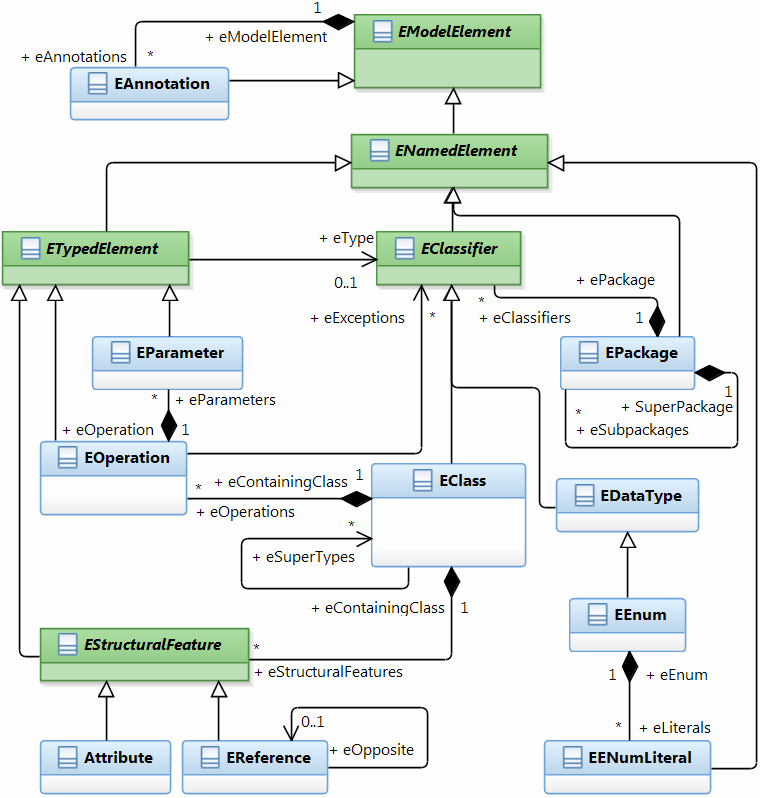
\includegraphics[scale=0.7]{images/ecore_metamodel.png}
  \caption{Ecore Metamodell (vereinfacht)}
  \label{fig:ecore_metamodel}
\end{figure}

% \newpage

\section{Henshin}

Der Name "`Henshin"' bedeutet Transformation auf Japanisch. Henshin ist eine auf EMF
basierende \textit{in-place} Transformationssprache für Ecore Modelle. Als \textit{in-place} werden
Transformationssprachen bezeichnet, die Änderungen direkt (zur Laufzeit) am Modell durchführen. Im
Gegensatz dazu würde eine \textit{out-place} Transformationssprache das Ursprungsmodell nicht
verändern und eine neue Instanz des Modells mit den durchgeführten Änderungen erzeugen.
Grundsätzlich kann Henshin aber ebenfalls als \textit{out-place} Transformationssystem verwendet
werden, indem man ein Modell in Henshin lädt, die Transformation durchführt und das Modell wieder an
einem anderen Ort abspeichert.

Weitere Informationen über Henshin sind in \cite{Arendt2010}, \cite{BES10} und unter
\cite{HENSHIN} zu finden. Die folgenden Abschnitte geben einen kurzen Überblick über die Henshin
Funktionalitäten.

\subsection{Regeln}

Henshin ist ein Graphersetzungssystem, dieses Konzept beruht auf der Graphentheorie. Ein Graph ist
in Henshin typisiert und besteht aus Knoten, gerichteten Kanten und Attributen. Eine Transformation
wird durch eine Regel angegeben. Diese Regel besteht aus einer linken (\textit{Left-Hand Site}
(LHS)) und einer rechten Seite (\textit{Right-Hand Site} (RHS)). Beide Seiten der Regel sind
Graphen. Der Grundgedanke bei Graph-Transformationsregeln ist ähnlich wie bei Produktionsregeln von
Chomsky-Grammatiken für Texte, es wird innerhalb des s.g. Arbeitsgraphen ein Bild gesucht, welches
der linken Seite entspricht. Man spricht auch von einer Abbildung (\textit{engl. Match}) oder im
Sinne der Graphentheorie von einem Graphmorphismus der linken Seite auf den Arbeitsgraphen. Wurde
eine solche Abbildung gefunden, dann wird diese durch die rechte Seite ersetzt.  Konnte die
Transformation korrekt durchgeführt werden, dann wird die Regel als anwendbar bezeichnet.
Zusätzlich muss noch der Schnitt von LHS und RHS angegeben werden. Dazu müssen in Henshin Mappings
zwischen allen LHS und RHS Knoten angelegt werden, die den gleichen Knoten repräsentieren. Der
Schnitt zwischen LHS und RHS ist genau der Teil der Abbildung, der beim Ausführen der Regel bewahrt
(also nicht verändert) wird. Alle Teile der linken Seite, die nicht im Schnitt enthalten sind,
werden also aus dem Arbeitsgraphen entfernt. Alle Teile der rechten Seite, die nicht im Schnitt
enthalten sind, werden im Gegensatz dazu neu in den Arbeitsgraphen eingefügt.

Um die Abbildungen einer Regel einzuschränken, können zusätzlich noch s.g. \textit{negativ
application conditions} (NAC) formuliert werden. Eine NAC ist ebenfalls ein Graph. Allerdings darf
sich dieser NAC Graph nicht auf den Arbeitsgraphen abbilden lassen, damit die Regel angewendet
werden darf. Mehrere NACs können über eine \texttt{AND} Formel logisch miteinander verbunden werden.

Für jeden Knoten können auch, entsprechend seinem Typ, Attribute angelegt werden. Jedes Attribut hat
einen bestimmten Wert. Der Wert eines Attributs kann entweder ein primitiver Wert sein oder ein
\textit{JavaScript} Ausdruck. Innerhalb des Ausdrucks können Parameter verwendet werden. Diese
werden einfach mit dem entsprechenden Namen für die Regel angelegt. Ein Parameter kann entweder beim
Aufrufen von außen an die Regel übergeben werden oder er wird beim Abbilden der linken
Seite mit einem Wert aus dem entsprechenden Objekt des Arbeitsgraphen initialisiert. Dazu muss es
mindestens ein Henshin Attribut auf der linken Seite der Regel geben, welches nur den Parameter
als Wert besitzt. Der Ausdruck wird dann durch die Rhino Script-Engine \cite{RIHNO}  verarbeitet und
ausgewertet.

Wird ein Attribut auf der rechten Seite der Regel für einen Knoten angelegt, so wird der Wert des
Attributs in das Objekt des Arbeitsgraphen geschrieben, auf welches der Knoten abgebildet wurde.
Wird ein Attribut hingegen auf der linken Seite angelegt, dann muss sich der Wert ebenfalls auf den
Arbeitsgraphen abbilden lassen, sofern das Attribut nicht wie zuvor beschrieben zur Initialisierung
eines Parameters verwendet wurde.

\begin{figure}[htb]
  \centering
  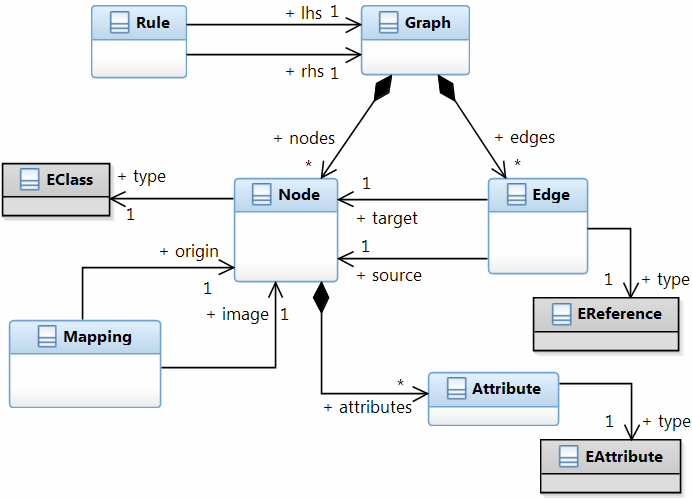
\includegraphics[scale=0.7]{images/henshin_metamodel.png}
  \caption{Henshin Metamodell für Regeln}
  \label{fig:henshin_metamodel}
\end{figure}

Das Henshin Metamodell, über welches die Regeln intern dargestellt werden, ist in Abbildung
\ref{fig:henshin_metamodel} zu sehen. Das Modell basiert auf Ecore und somit können beliebige
Modelle transformiert werden, die ebenfalls auf Ecore basieren.

\subsection{Units}

Mehrere Regeln werden in Henshin in Transforamtionssystemen zusammengefasst. Um den Ablauf einer
Transformation mit mehreren Regeln zu steuern, werden s.g. Units verwendet. Manche Units können auch
ineinander verschachtelt werden (siehe Abbildung \ref{fig:henshin_metamodel_units}). In diesem
Zusammenhang werden Regeln dann ebenfalls als Units betrachtet. Insgesamt wird in Henshin zwischen
sechs verschiedenen Units unterschieden. Eine Unit ist anwendbar, wenn sie erfolgreich ausgeführt
werden konnte. Wird festgestellt, dass eine Unit nicht anwendbar ist, dann werden alle
Transformationen, die bis zu diesem Zeitpunkt gemacht wurden, wieder rückgängig gemacht.

\begin{itemize}
  \item \textbf{Independent Unit:} Führt zufällig eine der Subunits einmal aus. Eine Idependent Unit
  ist anwenbar, wenn mindestens eine Subunit anwendbar ist.
  
  \item \textbf{Sequential Unit:} Führt alle Subunits in gegebener Reihenfolge aus. Eine Sequential
  Unit ist anwenbar, wenn alle Subunits anwendbar sind.
  
  \item \textbf{Counted Unit:} Führt die Subunit mit der angegebenen Häufigkeit aus. Mit einer
  Häufigkeit von -1 wird die Subunit solange ausgeführt, bis sie nicht mehr anwendbar ist. Eine
  Counted Unit mit einer Häufigkeit von -1 ist immer anwendbar, ansonsten ist die Counted Unit
  anwendbar, wenn sie mit der angegebenen Häufigkeit ausgeführt werden konnte.
  
  \item \textbf{Conditional Unit:} \texttt{IF THEN ELSE} Konstrukt für Units. Eine Conditional Unit
  ist anwendbar, wenn (je nach Anwendbarkeit der \texttt{IF} Subunit) die \texttt{THEN} Subunit bzw.
  die \texttt{ELSE} Subunit anwendbar ist.
 
  \item \textbf{Priority Unit:} Führt die erst mögliche anwendbare Subunit mit der höchsten Priorität
  einmal aus.
  
  \item \textbf{Amalgamation Unit:} Eine Amalgamation Unit besteht aus einer Kernregel und beliebig
  vielen Multiregeln. Die Kernregel wird dann genau einmal ausgeführt, während die Multiregeln
  so oft wie möglich ausgeführt werden. Damit die Amalgamation Unit anwendbar ist, muss mindestens
  die Kernregel anwendbar sein. Die Kernregel muss dabei in jede Multiregel eingebettet werden. Dies
  wird gekennzeichnet durch Mappings zwischen den Knoten der Kernregel und den entsprechenden
  Knoten der Multiregel.
\end{itemize}

\begin{figure}[h!]
  \centering
  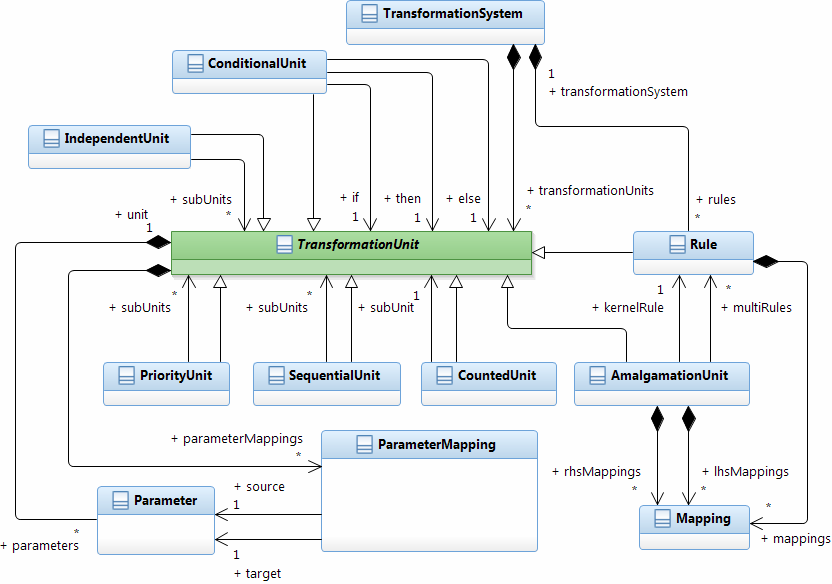
\includegraphics[width=1.0\textwidth]{images/henshin_metamodel_units.png}
  \caption{Henshin Metamodell für Units}
  \label{fig:henshin_metamodel_units}
\end{figure}

\subsection{Editoren}

Henshin bietet zwei Editoren zum Entwickeln von Transformationssystemen. Der erste Editor (Abbildung
\ref{fig:henshin_tree}) basiert auf dem Standard EMF-Editor und bietet eine baumbasierte Ansicht des
Transformationssystems. Der zweite Editor (Abbildung \ref{fig:henshin_rule}) ist speziell dazu
gemacht, um Henshin Regeln zu entwerfen. Die Regeln werden hier in einer integrierten Darstellung
angezeigt. D.h. alle Elemente (Knoten, Kanten, Attribute), die nur auf der linken Seite der Regel
vorkommen, werden mit dem Stereotyp \texttt{<<delete>>} gekennzeichnet; Alle Elemente, die nur auf
der rechten Seite der Regel vorkommen, werden mit \texttt{<<create>>} gekennzeichnet und alle
Elemente, die im Schnitt von LHS und RHS enthalten sind, werden mit \texttt{<<preserve>>}
gekennzeichnet. Der Graph der Regel lässt sich also intuitiv so lesen, dass alle \texttt{<<delete>>} Anteile gelöscht,
alle \texttt{<<create>>}  Anteile hinzugefügt und alle \texttt{<<preserve>>} Anteile bewahrt werden,
wenn die Regel auf den Arbeitsgraphen angewendet wird. NAC Anteile werden in dieser Darstellung
durch den Stereotyp \texttt{<<forbid>>} gekennzeichnet. Im Beispiel in Abbildung
\ref{fig:henshin_tree} und \ref{fig:henshin_rule} wird ein \texttt{EAttribute} von einer
\texttt{EClass} in ein über eine \texttt{EReference} benachbarte \texttt{EClass} verschoben.

\begin{figure}[h!]
  \centering
  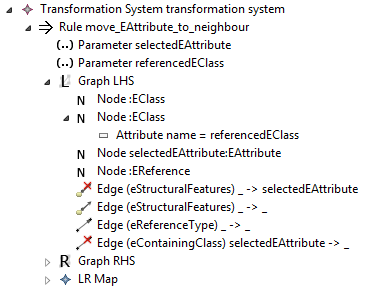
\includegraphics[scale=1.0]{images/henshin_tree.png}
  \caption{Baumbasierter Henshin Editor}
  \label{fig:henshin_tree}
\end{figure}

\begin{figure}[h!]
  \centering
  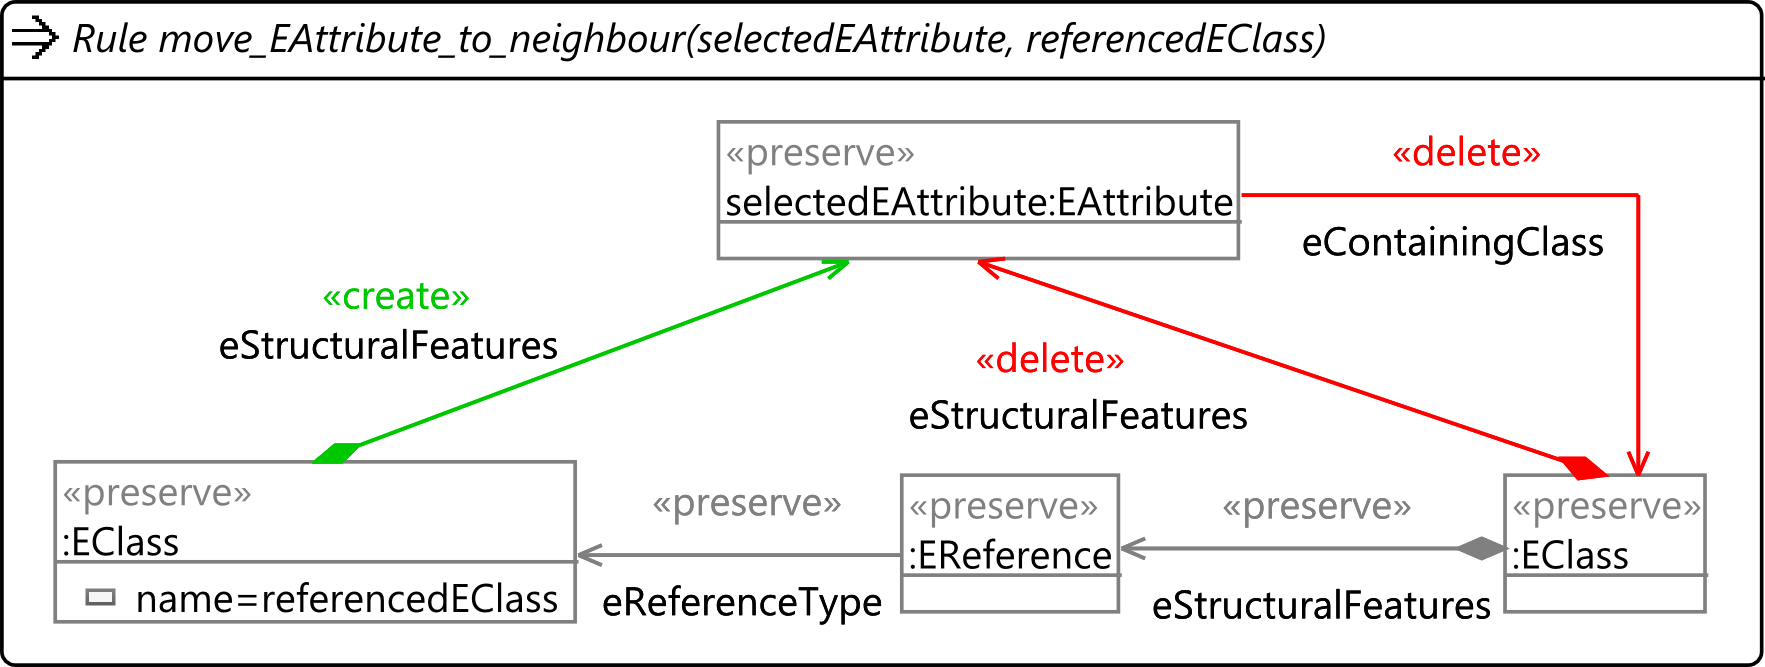
\includegraphics[width=1.0\textwidth]{images/henshin_rule.png}
  \caption{Visueller graphbasierter Henshin Editor}
  \label{fig:henshin_rule}
\end{figure}